\section{\tool Overview}
\label{sec:ex}
%$w^Tx>0$, mnist logistic regression
%% \divya{add reference to before and later... as mentioned we would run evaluations on secure prediction of different models. Here we describe scenario in detail..}

\begin{figure}
  %\vspace{-20pt}
  %\begin{center}
  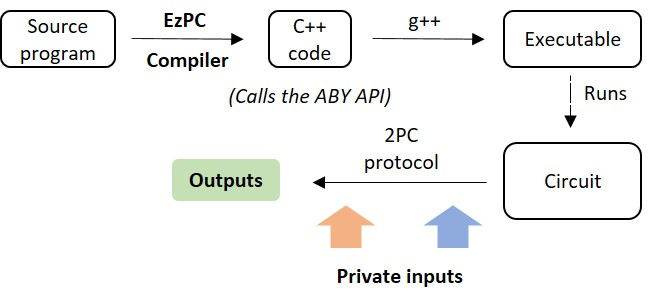
\includegraphics[width=0.45\textwidth]{toolchain}
  %\end{center}
  %\vspace{-20pt}
\caption{\tool toolchain}
\label{fig:toolchain}
\end{figure}

Figure~\ref{fig:toolchain} shows an overview of the \tool
toolchain. We give a brief overview of each of these phases below.

\subsubsection*{Source language}
Consider the example $w^Tx >b$ from Section~\ref{sec:intro}, where
$w$ and $b$ constitute the server's input (a classifier) and $x$ is
the client's input vector. Figure~\ref{fig:ex-sml} shows \tool code
for this example. The code first reads the inputs of the two parties
using the \ls{input1} and \ls{input2} expressions. It then uses a
\ls{for} loop to compute \ls{acc}, the dot product of \ls{w} and
\ls{x}. Finally, the code outputs the result of comparing \ls{acc}
with \ls{b} only to the client.

\tool source language is a simple, imperative language that enables
the programmers to express \mpc computations in terms of their
``ideal'' functionalities, without dealing with any cryptographic
details. The languages provides multi-dimensional arrays, conditional
expressions (the ternary $?\::$ operator), \ls{for}~loops,
\ls{if}~statements, and special syntax for input/output.

\begin{figure}
\begin{verbatim}
for (uint32_t i = 0; i < 30; i++)
{
    share * s_a_tmp_0 = acirc->
    					PutMULGate( s_a_a[i] , s_a_b[i] );
    s_a_j = acirc->
    		PutADDGate( s_a_j , s_a_tmp_0 );
}

share *s_y_j = ycirc->PutA2YGate( s_a_j );
uint32_t _tmp_2 = 1<<31-1 ;
share * s_y__tmp_2 = ycirc->PutCONSGate
					( _tmp_2 ,bitlen);
share * s_y_tmp_1 = ycirc->PutGTGate
					( s_y_j , s_y__tmp_2 );
uint32_t _tmp_3 = 1 ;
share * s_y__tmp_3 = ycirc->PutCONSGate
					( _tmp_3 ,bitlen);
uint32_t _tmp_4 = 0 ;
share * s_y__tmp_4 = ycirc->PutCONSGate
					( _tmp_4 ,bitlen);
share * s_y_k = ycirc->PutMUXGate
					( s_y__tmp_3 , s_y__tmp_4 , s_y_tmp_1 );
share * s_y_tmp_5 = ycirc->PutOUTGate
					( s_y_k , ALL);
party->ExecCircuit();
uint32_t _output = s_y_tmp_5->
			get_clear_value<uint32_t>();
\end{verbatim}
\caption{Code in ABY}
\label{fig:ex-aby}
\end{figure}

\subsubsection*{\tool compiler}
\tool compiler takes as input a source program and produces a C++
program as output. Figure~\ref{fig:ex-aby} shows the output code for
the example in Figure~\ref{fig:ex-sml}. The output program
contains party-specific code for inputs and outputs
(\ls{role == SERVER} and \ls{role == CLIENT}), and common code for the
computation.

The compiler splits the input
program into \emph{public} and \emph{secret} components. The public
components translate into regular C++ code, while the secret
components translate into API calls into our crypto back-end
(ABY). For instance, for the code in Figure~\ref{fig:ex-sml}, the \tool
compiler realizes that the array index \ls{i} in the dot product loop
is public, and hence the array accesses need not be compiled
obliviously. Therefore, it compiles the \ls{for}~loop into a C++
\ls{for}~loop that will be executed in-clear
(line~\ref{line:dotproductloop}).

Within the secret components, the \tool compiler is ``cryptographic
cost-aware'', and appropriately picks either arithmetic or boolean
circuit representations for different sub-componenets. For example,
the compiler realizes that the dot product computation is more
efficient in the arithmetic representation, and therefore it builds
the corresponding circuit using the arithmetic circuit builder
\ls{acirc} (lines~\ref{line:dotmulgate} and~\ref{line:dotaddgate}). On
the other hand, since the comparison with \ls{b}, and the conditional
expression computation are more efficient in the boolean
representation, the \tool compiler uses the Yao circuit builder
\ls{ycirc} to build the corresponding circuits
(lines~\ref{line:condyaobegin} to~\ref{line:condyaoend})\footnote{As
  we mention in
  Section~\ref{sec:impl}, in our usage of ABY, boolean is synonymous
  with Yao.}.

Importantly, conversions between the arithmetic and boolean
represenation require share-conversions. The \tool compiler also
instruments these conversion gates accordingly. For example, in
lines~\ref{line:convacc} and~\ref{line:convb}, the compiler converts
\ls{a_acc} and \ls{a_b} to boolean representation, before they are
input to the comparison and multiplexer circuits.

\subsubsection*{Circuit generation and evaluation} The next step in
\tool is to
compile the output C++ code and execute it. Doing so reduces away the
public parts of the program, including the array accesses, and
generates a \mpc circuit comprising of arithmetic and boolean gates,
with appropriate conversion gates. The circuit is then evaluated using
a \mpc protocol.

We can now concretely see the advantages of \tool. Unarguably, it is
easier for a developer to program, and get right, the code in
Figure~\ref{fig:ex-sml}, rather than the code in
Figure~\ref{fig:ex-aby} (as we mentioned in Section~\ref{sec:intro},
other high-level languages are limited in their use of a single,
arithmetic or boolean, crypto back-end). \tool also enables the
programmer to easily modify their code, while the compiler takes care
of efficiency. For example, consider in Figure~\ref{fig:ex-sml} a
change from multiplication to bitwise OR in the \ls{for} loop. It
turns out that once that's the case, it is more efficient to do both
the addition and bitwise OR using boolean circuits (if the addition is
still done using arithmetic, the conversion cost starts to take
over). In \tool, the programmer simply needs to change one operator in
the source code, and the compiler generates efficient code that uses
boolean addition. Whereas, if the programmer was writing ABY
code, she either has to sacrifice performance, or she would have to
revisit many parts of the circuit and change them.

To summarize, \tool raises the level of abstraction for the
programmers, and generates efficient crypto protocols automatically,
while its metatheory provides strong correctness and security
guarantees.

%% Consider a  cloud service provider Bob that wants to provide a service to diagnose
%% whether a patient has breast cancer or not. Bob trains a machine learning classification model
%% that results in a vector $w$ (say of length 30) and a scalar $b$.
%% This model is the intellectual property of Bob and he  wants to keep it secret.
%% Given a patient's medical report, in the form of a vector $x$ (also of length 30),
%% the classifer predicts that the patient has breast cancer if $w^Tx>b$.
%% However, for this task Bob needs access to $x$, which is private data of a customer.

%% A potential customer Alice might not want to reveal $x$ to Bob because of privacy concerns.
%% And Bob does not want to reveal $w$ and $b$ because then Alice can steal the model. \divya{Use HIPAA compliance; as it can leak information of patients that was used in training; more compelling argument. See Shafi intro.}
%% SMC can help Alice and Bob compute $w^Tx>b$ securely, such that Alice receives the classifier's
%% prediction and Bob learns nothing about $x$. Moreover, Alice does not learn anything more about $w$
%% and $b$ than what is revealed by the prediction. 
%% \nc{This is a bit repetitive from the intro, isnt it? Should we have another example perhaps?}
%% To implement this system, Bob can write the code in \tool and this code is shown in Figure~\ref{fig:ex-sml}.
%% The expression {\tt input1} reads a value from Bob and {\tt input2} reads from Alice.
%% The language has arrays and simple loops. A loop {\tt for i = [0:N]} repeats its
%% body {\tt N} times, the loop counter {\tt i} is assigned {\tt 0} in the first iteration,
%% and is incremented by one after each iteration. Unbounded {\tt while} loops are problematic
%% from a cryptographic standpoint and our language only permits these simple {\tt for} loops. 
%% The first loop in Figure~\ref{fig:ex-sml} reads the model $w$ from Bob, the second loop reads
%% Alice's medical report $x$, and the third loop computes the dot product $w^Tx$.
%% The last {\tt output} statement sends the result of the comparison $w^Tx>b$ to Alice.
%% In particular, the ternary ``{\tt ? :}" operator performs a branch and the result is the second (third)
%% argument if the first argument is true (false).

%% The \tool compiler is fully automatic and compiles the code described in Figure~\ref{fig:ex-sml} to the C++ code that makes calls to the ABY library  in
%% Figure~\ref{fig:ex-aby}. An alternative to using \tool is to directly write this C++ code.
%% However, this code is much more complex than the implementation written in \tool.
%% Therefore, it is difficult for Alice and bob to verify its correctness and security.
%% Unlike \tool implementations, the ``secret" variables containing private data ({\tt w,x,b,acc}) need to be handled differently compared to ``public" variables such as loop counters ({\tt i}). In particular, the former are manipulated by the ABY library and the latter are manipulated like standard  C++ variables.
%% Additionally, the C++ code branches on  the special variable
%% {\tt role}  to decide whether the enclosing code is executed by the {\tt SERVER} Bob or by
%% the {\tt CLIENT} Alice. In Figure~\ref{fig:ex-sml}, the developer does not need to
%% manipulate {\tt role} explicitly. In addition to simplifying the implementation, \tool prevents developers from writing buggy code such as\\
%% \verb+if(role == SERVER) {...manipulate x...}+

%% Furthermore, the code in Figure~\ref{fig:ex-aby} is too low level.
%% In particular, it is first builds a circuit that represents the computation
%% $w^Tx>b$ and then executes it via a call to {\tt ExecCircuit}.
%% To build a circuit, the code adds multiplication gates ({\tt PutMULGate})
%% and addition gates ({\tt PutADDGate}) for the dot product.
%% Subsequently, it uses a ``greater than" gate ({\tt PutGTGate})
%% and a multiplexer gate ({\tt PutMUXGate}) for the comparison with $b$.
%% For efficiency, the operations for dot product need to be performed using 
%% arithmetic circuits. However, ABY's arithmetic circuits cannot express
%% comparisons and these need  boolean circuits.
%% A program that uses both arithmetic circuit and boolean circuits
%% requires conversion gates that help  interconvert between arithmetic
%% representations and boolean representations ({\tt PutA2YGate}).
%% Bigger computations often require multiple conversions and the
%% developer effort can quickly become significant.

%% Moreover, it is difficult to maintain the code in Figure~\ref{fig:ex-aby}.
%% For example, if the multiplication is changed to a bitwise-or then,
%% in the absence of \tool, an efficiency-conscious developer would need to  use boolean circuits everywhere and would be tasked with removing all arithmetic circuits and the interconversion gates (the cost of  conversion overweighs the gains of performing an arithmetic addition instead of a boolean addition). 
%%  With \tool, the developer needs to change only a single character (replace {\tt *} in Figure~\ref{fig:ex-sml} with {\tt |}) to achieve the same effect. 
%% On this example and other small examples, we have found that the compiler generated C++ code from a \tool implementation is as efficient as manually written C++ code. In particular, for $w^Tx>b$, the compiler automatically generates code that uses arithmetic circuits for dot product and inserts appropriate conversion gates. Finally, although this paper uses ABY for evaluation, the  compiler can be easily retargeted to generate code for other cryptography backends.


%% The \tool compiler provides strong static guarantees. For example, a well typed
%% \tool program is guaranteed to execute to termination without errors. A \tool program cannot go into non-termination or dereference illegal memory, i.e., no buffer overflows or underflows can happen at run time. Production compilers such as {\tt gcc} provide no such guarantees
%% for the code in Figure~\ref{fig:ex-aby}.
%% The primary reason that we are able to achieve these guarantees is because
%% \tool has been designed to be verifiable and is backed by formal semantics. 
%% Furthermore, the compiler output is guaranteed to be a cryptographically secure
%% implementation of the functionality declared by the \tool code. 
%% Moreover, the \tool compiler also generates a C implementation that can be run natively on a single machine for functional testing. 

